\documentclass[journal]{IEEEtran}
\usepackage{amsmath,amsfonts}
\usepackage{algorithmic}
\usepackage{algorithm}
\usepackage{amssymb}
\usepackage{array}
\usepackage[caption=false,font=normalsize,labelfont=sf,textfont=sf]{subfig}
\usepackage{textcomp}
\usepackage{stfloats}
\usepackage{url}
\usepackage{verbatim}
\usepackage{graphicx}
\usepackage{cite}
\usepackage{xcolor}
\hyphenation{op-tical net-works semi-conduc-tor IEEE-Xplore}

% updated with editorial comments 8/9/2021
% not show the red box
\usepackage[hidelinks]{hyperref}

\usepackage{booktabs} % for \hline
\renewcommand{\algorithmicrequire}{\textbf{Input:}}
\renewcommand{\algorithmicensure}{\textbf{Output:}}
\usepackage{threeparttable}
\usepackage{amsthm}
\newtheorem{definition}{Definition}
\newtheorem{proposition}{Proposition}
\usepackage{listings}


\begin{document}

\title{High Throughput Implementation of AES on GPUs} 


\author{Jiahao Xiang and Lang Li.
        % <-this % stops a space

\thanks{This work is supported by the Hunan Provincial Natural Science Foundation of China (2022JJ30103), Postgraduate Scientific Research Innovation Project of Hunan Province (CX20240977), “the 14th Five-Year Plan” Key Disciplines and Application-oriented Special Disciplines of Hunan Province (Xiangjiaotong [2022] 351), the Science and Technology Innovation Program of Hunan Province (2016TP1020).}


\thanks{Jiahao Xiang and Lang Li are with the Hunan Provincial Key Laboratory of Intelligent Information Processing and Application, Hengyang Normal University, Hengyang 421002, China, and also with the College of Computer Science and Technology, Hengyang Normal University, Hengyang 421002, China (e-mail: jiahaoxiang2000@gmail.com; lilang911@126.com).}% <-this % stops a space
}
% \thanks{Manuscript received April 19, 2021; revised August 16, 2021.}}
% \thanks{Manuscript received }}

% The paper headers
\markboth{Journal of \LaTeX\ Class Files,~Vol.~14, No.~8, August~2021}%
{Shell \MakeLowercase{\textit{et al.}}: A Sample Article Using IEEEtran.cls for IEEE Journals}

\IEEEpubid{}
% Remember, if you use this you must call \IEEEpubidadjcol in the second
% column for its text to clear the IEEEpubid mark.

\maketitle


\begin{abstract}
   \textcolor{blue}{The rapid increase in data transfer rates from gigabits per second to terabits per second necessitates efficient computational approaches for high-speed data processing. Traditional software and extended instruction set architectures prove inadequate under these conditions. A GPU-based software implementation of the AES is presented, employing bitslicing to compute substitutions on the fly and thereby reducing cache misses compared with look-up table methods. Additional gains are realized through a permutation optimization that mitigates thread stall time. Experimental results indicate that this implementation achieves throughput in xx.xx terabit-per-second when executed on a single NVIDIA RTX 4090 GPU.
   } 
    
\end{abstract}

\begin{IEEEkeywords}
   Software implementation, Block cipher, GPU, Bitslicing, SAT.
\end{IEEEkeywords}

\color{blue}
\section{Introduction}
\label{sec:intro}

% Growing data volumes necessitate high-throughput encryption schemes to ensure data confidentiality. The Advanced Encryption Standard (AES) remains the most prominent block cipher, with software implementations commonly adopted for flexibility and scalability. 


\IEEEPARstart{T}{he} Advanced Encryption Standard (AES) is a widely adopted symmetric block cipher that provides essential security in diverse communication protocols \cite{Daemen2020}. Commonly used libraries such as OpenSSL and Libgcrypt employ T-table-based methods for both encryption and decryption, delivering adequate performance for megabit-per-second workloads \cite{Jancar2024, Marshall2021}.

Performance shortcomings arise when data rates exceed gigabit-per-second thresholds \cite{Li2020}. Such high-throughput scenarios, including data centers and 5G networks, require more efficient and scalable solutions to preserve both speed and cryptographic strength.

\subsection{Related Work}

The parallel structure of GPUs supports the simultaneous execution of multiple threads, which significantly increases performance in comparison with standard CPU-based operations. Table~\ref{tab:relared_work} summarizes representative AES CTR mode implementations on GPUs. In \cite{Hajihassani2019}, the overhead of the ShiftRows stage is minimized by rearranging input data, and a hardware-based S-box replaces look-up table resources in the Substitute Bytes stage. In \cite{Lee2022}, the necessity to embed round keys at compile time is eliminated, allowing more flexible code generation. This approach achieves 9\% higher encryption throughput than bit-sliced references for CTR modes.

\begin{table}
    \caption{Related Work on AES CTR mode Implementations on GPUs}
    \label{tab:relared_work}
    \centering
    \begin{tabular}{cccc}
        \toprule
        \textbf{Ref} & \textbf{Throughput (Gbps)} & \textbf{Platform} & \textbf{Year} \\
        \midrule
        \cite{Hajihassani2019} & 1478 & Tesla V100 & 2019 \\
        \cite{Lee2022}        & 1489 & RTX 3080   & 2022 \\
        Ours     & --   & RTX 4090         & --   \\
        \bottomrule
    \end{tabular}
\end{table}

\subsection{Motivation}


\subsection{Contributions}



\color{black}

% \section*{Acknowledgments}


% {\appendix[Proof of the Zonklar Equations]
% Use $\backslash${\tt{appendix}} if you have a single appendix:
% Do not use $\backslash${\tt{section}} anymore after $\backslash${\tt{appendix}}, only $\backslash${\tt{section*}}.
% If you have multiple appendixes use $\backslash${\tt{appendices}} then use $\backslash${\tt{section}} to start each appendix.
% You must declare a $\backslash${\tt{section}} before using any $\backslash${\tt{subsection}} or using $\backslash${\tt{label}} ($\backslash${\tt{appendices}} by itself
%  starts a section numbered zero.)}



%{\appendices
%\section*{Proof of the First  Equation}
%Appendix one text goes here.
% You can choose not to have a title for an appendix if you want by leaving the argument blank
%\section*{Proof of the Second  Equation}
%Appendix two text goes here.}


 % argument is your BibTeX string definitions and bibliography database(s)
\bibliography{biblio}

\bibliographystyle{IEEEtran}


% \newpage


% \bf{If you include a photo:}\vspace{-33pt}
\begin{IEEEbiography}[{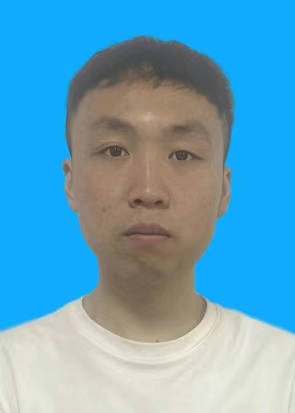
\includegraphics[width=1in,height=1.25in,clip,keepaspectratio]{./fig/slef.jpg}}]{Jiahao Xiang}
    is pursuing a Master's degree in Electronic Information at Hengyang Normal University, China. His research focuses on cryptographic engineering and efficient implementations of block ciphers on resource-constrained devices. Publications include works on lightweight cryptography optimization and contributions to open-source cryptographic projects.
\end{IEEEbiography}

\begin{IEEEbiography}[{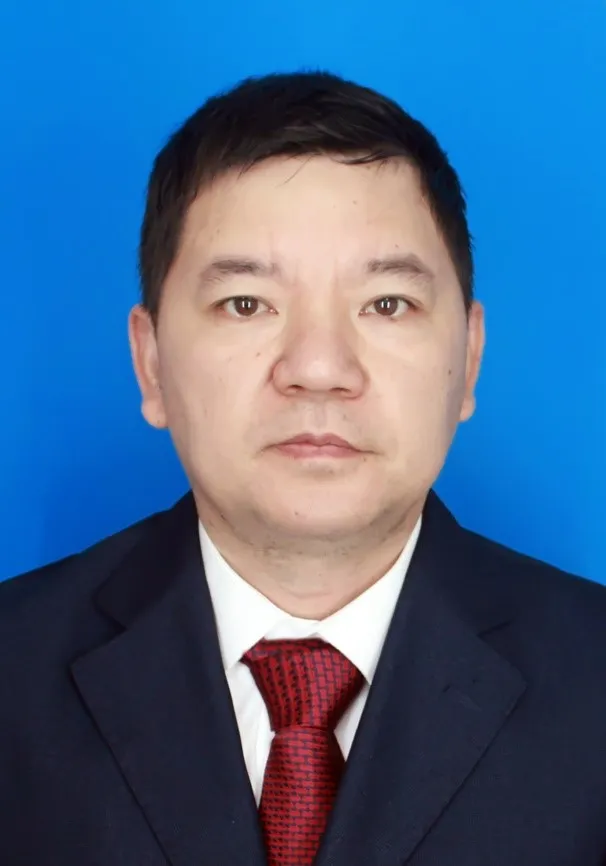
\includegraphics[width=1in,height=1.25in,clip,keepaspectratio]{./fig/boss.png}}]{Lang Li}
    received his Ph.D. and Master's degrees in computer science from Hunan University, Changsha, China, in 2010 and 2006, respectively, and earned his B.S. degree in circuits and systems from Hunan Normal University in 1996. Since 2011, he has been working as a professor in the College of Computer Science and Technology at the Hengyang Normal University, Hengyang, China. He has research interests in embedded system and information security.  
\end{IEEEbiography}

% \vspace{11pt}

% \bf{If you will not include a photo:}\vspace{-33pt}
% \begin{IEEEbiographynophoto}{Jiahao Xiang}
% is pursuing a Master's degree in Electronic Information at Hengyang Normal University, China. His research focuses on cryptographic engineering and efficient implementations of block ciphers on resource-constrained devices. Publications include works on lightweight cryptography optimization and contributions to open-source cryptographic projects.
% \end{IEEEbiographynophoto}

% \begin{IEEEbiographynophoto}{Lang Li}
%  received his Ph.D. and Master's degrees in computer science from Hunan University, Changsha, China, in 2010 and 2006, respectively, and earned his B.S. degree in circuits and systems from Hunan Normal University in 1996. Since 2011, he has been working as a professor in the College of Computer Science and Technology at the Hengyang Normal University, Hengyang, China. He has research interests in embedded system and information security.  
% \end{IEEEbiographynophoto}



\vfill

\end{document}


